
\chapter{背景分析}

勇者闯迷宫对应到现实生活中的场景是最简单的寻路算法,寻路算法是一种应用广泛且十分重要的算法,%
它的主要应用场景有:导航、搜索路径、地形分析、网络路由以及在游戏中的自动寻路。可以说,寻路算法渗透了%
我们生活的方方面面,实现一个正确且快速的寻路算法对实际场景有着重要意义。

通过简单场景模拟寻路是探究寻路算法的好方式,本项目通过一个迷宫场景来构建路径和障碍物的关系,%
在模拟中,项目采用了回溯法进行路径的求解,遇到障碍就会回头,以确保在失败前探索所有可能的路径。%

{\kaishu 深度优先搜索(Deep First Search, DFS)}算法是回溯法的一种实现方式,本项目也是用 \emph{DFS}%
实现的。相较于简单的递归实现,我在项目中采用了迭代法实现,提高了项目能承载数据的上限,不用担心函数调用栈溢出问题。

\begin{figure}[H]
    \tikzstyle{c} = [minimum width = 8mm, minimum height = 8mm, draw = black, fill = black, text = white]
    \tikzstyle{p} = [minimum width = 8mm, minimum height = 8mm, draw = black, fill = white]
    \tikzstyle{s} = [minimum width = 8mm, minimum height = 8mm, draw = black, fill = red]
    \centering
    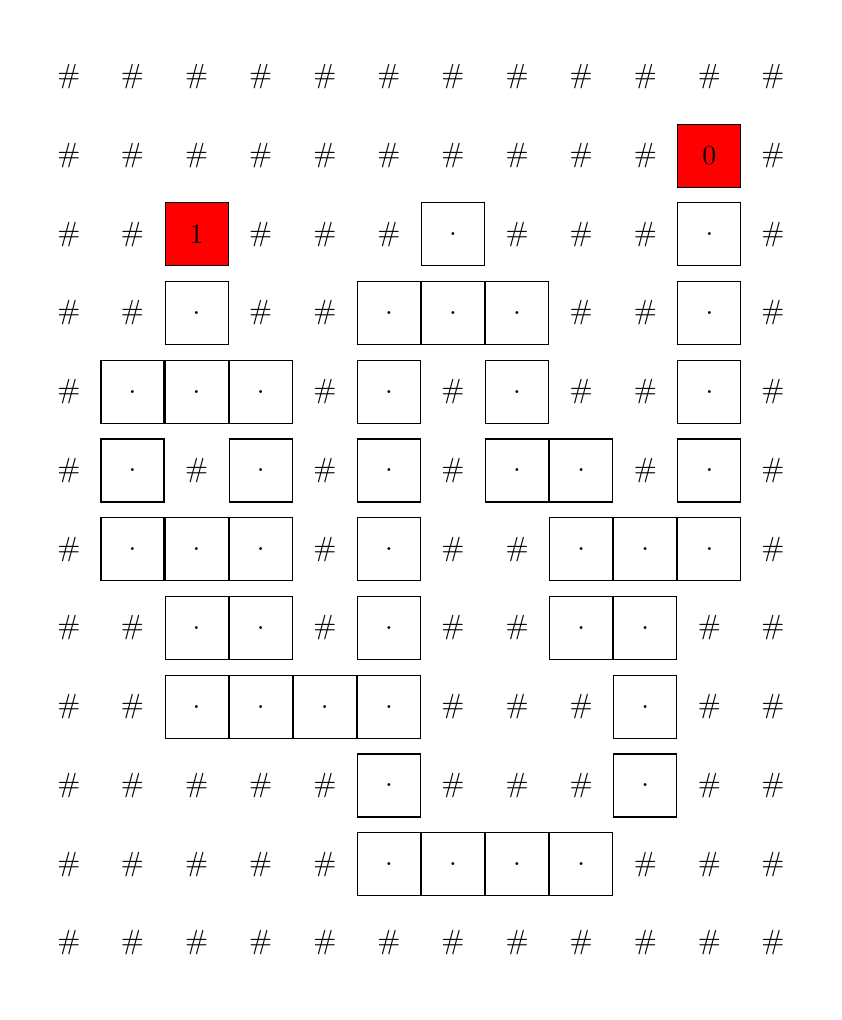
\begin{tikzpicture}
        \matrix (maze) [draw = white]
        {
            \node [c] {\#}; & \node [c] {\#}; & \node [c] {\#}; & \node [c] {\#}; & \node [c] {\#}; & \node [c] {\#}; & \node [c] {\#}; & \node [c] {\#}; & \node [c] {\#}; & \node [c] {\#}; & \node [c] {\#}; & \node [c] {\#};\\
            \node [c] {\#}; & \node [c] {\#}; & \node [c] {\#}; & \node [c] {\#}; & \node [c] {\#}; & \node [c] {\#}; & \node [c] {\#}; & \node [c] {\#}; & \node [c] {\#}; & \node [c] {\#}; & \node [s] {0};  & \node [c] {\#};\\
            \node [c] {\#}; & \node [c] {\#}; & \node [s] {1};  & \node [c] {\#}; & \node [c] {\#}; & \node [c] {\#}; & \node [p] {.};  & \node [c] {\#}; & \node [c] {\#}; & \node [c] {\#}; & \node [p] {.};  & \node [c] {\#};\\
            \node [c] {\#}; & \node [c] {\#}; & \node [p] {.};  & \node [c] {\#}; & \node [c] {\#}; & \node [p] {.};  & \node [p] {.};  & \node [p] {.};  & \node [c] {\#}; & \node [c] {\#}; & \node [p] {.};  & \node [c] {\#};\\
            \node [c] {\#}; & \node [p] {.};  & \node [p] {.};  & \node [p] {.};  & \node [c] {\#}; & \node [p] {.};  & \node [c] {\#}; & \node [p] {.};  & \node [c] {\#}; & \node [c] {\#}; & \node [p] {.};  & \node [c] {\#};\\
            \node [c] {\#}; & \node [p] {.};  & \node [c] {\#}; & \node [p] {.};  & \node [c] {\#}; & \node [p] {.};  & \node [c] {\#}; & \node [p] {.};  & \node [p] {.};  & \node [c] {\#}; & \node [p] {.};  & \node [c] {\#};\\
            \node [c] {\#}; & \node [p] {.};  & \node [p] {.};  & \node [p] {.};  & \node [c] {\#}; & \node [p] {.};  & \node [c] {\#}; & \node [c] {\#}; & \node [p] {.};  & \node [p] {.};  & \node [p] {.};  & \node [c] {\#};\\
            \node [c] {\#}; & \node [c] {\#}; & \node [p] {.};  & \node [p] {.};  & \node [c] {\#}; & \node [p] {.};  & \node [c] {\#}; & \node [c] {\#}; & \node [p] {.};  & \node [p] {.};  & \node [c] {\#}; & \node [c] {\#};\\
            \node [c] {\#}; & \node [c] {\#}; & \node [p] {.};  & \node [p] {.};  & \node [p] {.};  & \node [p] {.};  & \node [c] {\#}; & \node [c] {\#}; & \node [c] {\#}; & \node [p] {.};  & \node [c] {\#}; & \node [c] {\#};\\
            \node [c] {\#}; & \node [c] {\#}; & \node [c] {\#}; & \node [c] {\#}; & \node [c] {\#}; & \node [p] {.};  & \node [c] {\#}; & \node [c] {\#}; & \node [c] {\#}; & \node [p] {.};  & \node [c] {\#}; & \node [c] {\#};\\
            \node [c] {\#}; & \node [c] {\#}; & \node [c] {\#}; & \node [c] {\#}; & \node [c] {\#}; & \node [p] {.};  & \node [p] {.};  & \node [p] {.};  & \node [p] {.};  & \node [c] {\#}; & \node [c] {\#}; & \node [c] {\#};\\
            \node [c] {\#}; & \node [c] {\#}; & \node [c] {\#}; & \node [c] {\#}; & \node [c] {\#}; & \node [c] {\#}; & \node [c] {\#}; & \node [c] {\#}; & \node [c] {\#}; & \node [c] {\#}; & \node [c] {\#}; & \node [c] {\#};\\
        };
    \end{tikzpicture}
    \caption{迷宫示意图}
\end{figure}

\chapter{功能设计}

\section{题意转化}

本项目模拟的是骑士在迷宫中不断探路、受阻、返回,直到找到终点的过程,在项目功能要求里也有详细描述:

\begin{quote}
    \kaishu
    迷宫问题的求解过程可以采用回溯法即在一定的约束条件下试探地搜索前进,若前进中受阻,%
    则及时回头纠正错误另择通路继续搜索的方法。从入口出发,按某一方向向前探索,若能走通,%
    即某处可达,则到达新点,否则探索下一个方向;若所有的方向均没有通路,则沿原路返回前一点,%
    换下一个方向再继续试探,直到所有可能的道路都探索到,或找到一条通路,或无路可走又返回入口点。
\end{quote}

本项目采用的{\kaishu 深度优先搜索(Deep First Search, DFS)}算法在递归实现中十分简单:只需要在每一次进入某一个位置时记录该位置已走过,%
然后进入与该位置相邻的没有走过的位置,如果不存在这样的位置就函数返回,退回到上一个位置的函数状态。如此往复直到遇到是终点的位置。

但是递归法有其局限性:当函数调用栈的深度超过一定数量时,就有{\kaishu 栈溢出}(或俗称“爆栈”)的风险,这样的最大深度取决于电脑内存等因素,%
因为每次函数调用都要保存当时程序的环境,因此递归调用一次比迭代一次产生的新数据必然多几倍,是不推荐的解决方案。

接下来展示迭代算法的思路:


\section{逻辑功能}

\begin{enumerate}
    \item 用迷宫等大的二维数组表示一个的状态:未访问、待标记、死路。初始化成全部未访问。
    \item 用一个栈来储存当前探索过的位置。
    \item 从开始位置开始,对于每一个位置:
    \begin{enumerate}
        \item 如果当前位置是终点,退出循环。如果栈为空,也退出循环。
        \item 按照“上下左右”的顺序访问第一个相邻的没被访问的位置。置该位置“待标记”,并将位置入栈。
        \item 当前位置置为最新入栈的位置。
        \item 如果当前相邻位置没有可以进入的位置了,就置当前位置“死路”,栈顶弹出一个元素,再从栈顶取出一个位置置入当前位置。
    \end{enumerate}
    \item 结束后,如果栈为空,则返回 \lstinline{false},其他情况返回\lstinline{true}。
\end{enumerate}


用这种方法产生的路径与递归法产生的路径是相同有效的,可以说,迭代法产生了正确且更普适的实现。

此外,本项目使用的数据结构是{\kaishu 栈},栈是一种限定在{\kaishu 栈顶}做插入和删除操作的顺序表,其数据改变的特性是:%
{后进先出(Last In First Out, LIFO)},栈与函数调用有着密切的关系。

\begin{figure}[H]
    \centering
    \tikzstyle{c} = [minimum width = 8mm, minimum height = 10mm]
    \tikzstyle{token} = [draw = white, node distance = 1.2cm]
    \tikzstyle{arr} = [thick, ->]
\begin{tikzpicture}[every node/.style={draw}]
    \matrix (m1) [draw=white]
    {
          \node [c](1){1}; & \node [c](2){2}; & \node [c](3){3}; & \node [c](4){4}; & 
          \node [c](5){5}; & \node [c](6){6}; & \node [c](7){7}; & \node [c](8){ };\\
    };
    
    \node (r1)[token, above of = 7] {top};
    \draw [arr] (r1) -- (7);
    
    \matrix (m2) [draw=white, below of = m1, node distance = 2.3cm]
    {
          \node [c](21){1}; & \node [c](22){2}; & \node [c](23){3}; & \node [c](24){4}; & 
          \node [c](25){5}; & \node [c](26){6}; & \node [c](27){7}; & \node [c](28){8};\\
    };
    
    \node (r2)[token, above of = 28]{top};
    \draw [arr] (r2) -- (28);
    
    \matrix (m3) [draw=white, below of = m2, node distance = 2.3cm]
    {
          \node [c](31){1}; & \node [c](32){2}; & \node [c](33){3}; & \node [c](34){4}; & 
          \node [c](35){5}; & \node [c](36){6}; & \node [c](37){ }; & \node [c](38){ };\\
    };
    
    \node (r3)[token, above of = 36]{top};
    \draw [arr] (r3) -- (36);

    \matrix (m4) [draw=white, below of = m3, node distance = 2.3cm]
    {
          \node [c](41){1}; & \node [c](42){2}; & \node [c](43){3}; & \node [c](44){4}; & 
          \node [c](45){5}; & \node [c](46){ }; & \node [c](47){ }; & \node [c](48){ };\\
    };
    
    \node (r4)[token, above of = 45]{top};
    \draw [arr] (r4) -- (45);


\end{tikzpicture}
\caption{栈内部数据示意图\\}
\end{figure}